% ============================================================
% Figure Captions: Composition-Inflation in Bounded Phase Space
% ============================================================

\begin{figure*}[!htbp]
    \centering
    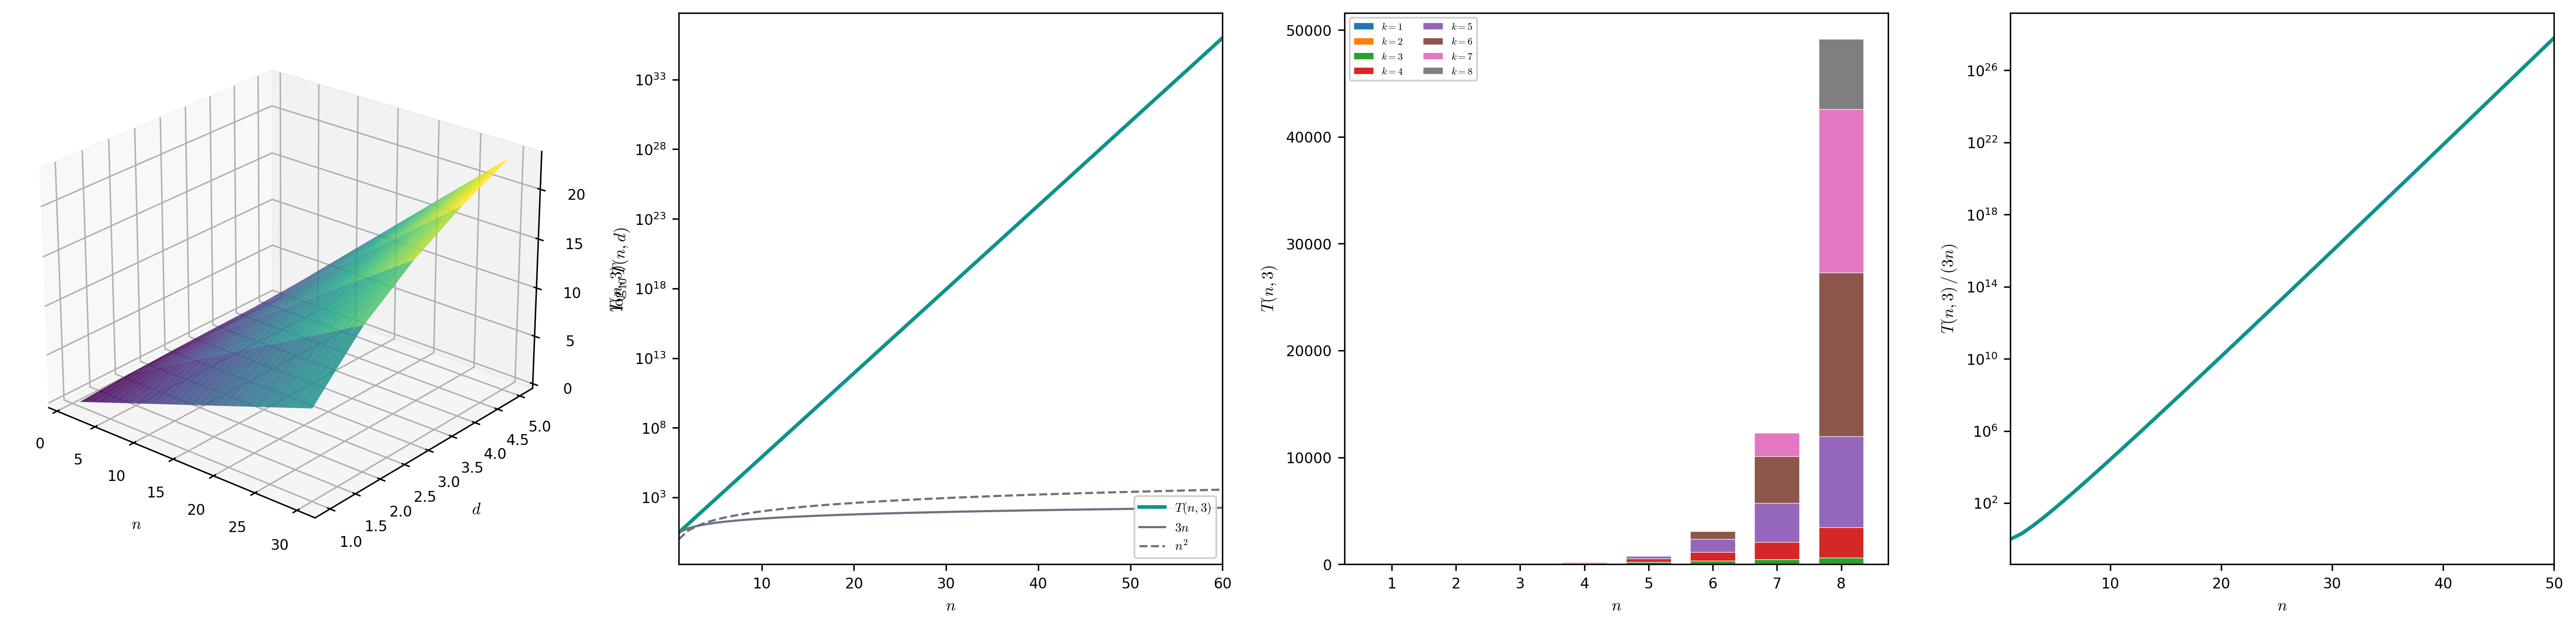
\includegraphics[width=\textwidth]{figures/panel_1_composition_growth.png}
    \caption{\textbf{Composition-Inflation Growth.}
    (\textbf{A})~Three-dimensional surface of $T(n,d) = d \cdot (d+1)^{n-1}$ over the $(n, d)$ plane for $n = 1, \ldots, 30$ and $d = 1, \ldots, 5$. The surface is coloured by $\log_{10} T$, transitioning from cool (low) to warm (high). The exponential dependence on $n$ produces a steeply rising surface, with higher-dimensional entropy spaces ($d = 4, 5$) climbing faster due to the larger exponential base $(d+1)$. Even at $n = 30$, the trajectory count exceeds $10^{17}$ for $d = 3$.
    (\textbf{B})~Semilogarithmic comparison of three growth regimes for $d = 3$: composition-inflated $T(n,3) = 3 \cdot 4^{n-1}$ (teal, exponential), linear $3n$ (grey, flat on log scale), and quadratic $n^2$ (grey dashed). The exponential dominance is immediate: by $n = 10$, $T$ exceeds $3n$ by a factor of $10^4$; by $n = 50$, the factor exceeds $10^{28}$. The linear and quadratic curves are indistinguishable from zero on this scale beyond $n \approx 15$.
    (\textbf{C})~Stacked bar decomposition of $T(n,3)$ by composition part count $k$ for $n = 1, \ldots, 8$. Each bar is partitioned into layers: $k = 1$ (compositions with a single part, contributing $3^1 = 3$ trajectories), $k = 2$ (contributing $\binom{n-1}{1} \cdot 3^2$), up to $k = n$ (contributing $3^n$). The highest-$k$ layer (all single-step compositions) dominates for large $n$, as $3^n$ grows faster than $\binom{n-1}{k-1} \cdot 3^k$ for fixed $k < n$. The total height equals $3 \cdot 4^{n-1}$.
    (\textbf{D})~Inflation factor $T(n,3)/(3n)$ versus $n$ on semilogarithmic scale. This ratio measures how many times more trajectories the composition-inflation mechanism produces compared to the naive linear count. The ratio grows as $4^{n-1}/n$, exceeding $10^{10}$ by $n = 20$ and $10^{28}$ by $n = 50$. The $n = 56$ mark (Planck depth for caesium) is annotated, where the inflation factor reaches $\sim 10^{32}$.}
    \label{fig:composition_growth}
\end{figure*}

\begin{figure*}[!htbp]
    \centering
    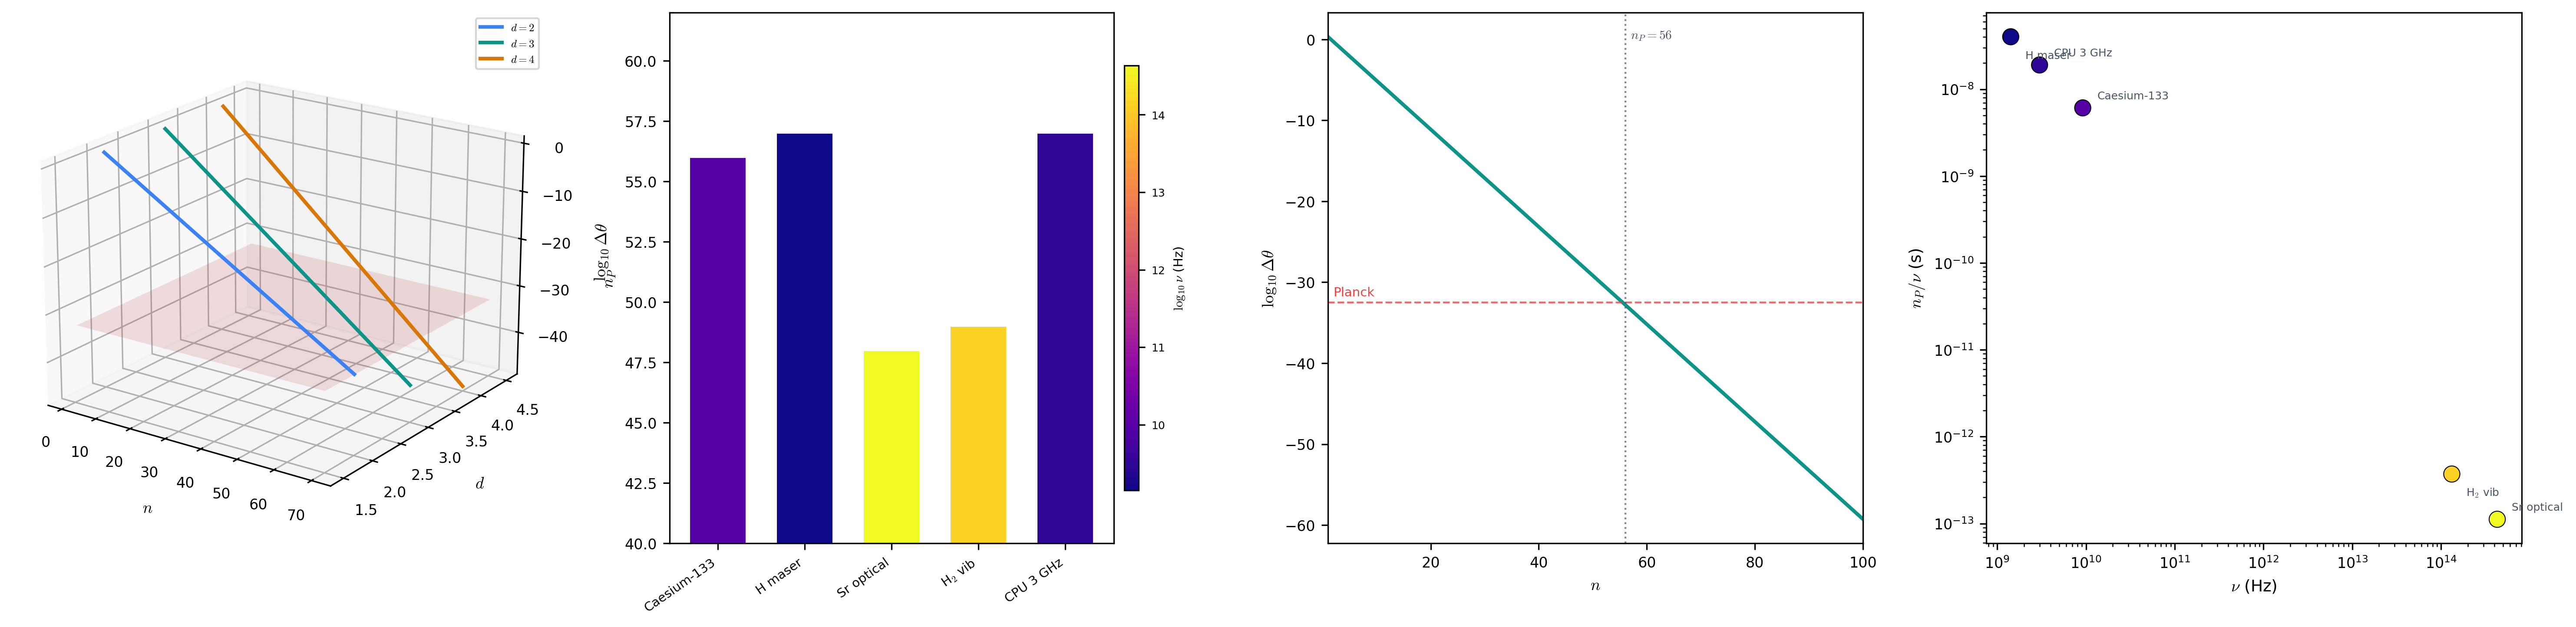
\includegraphics[width=\textwidth]{figures/panel_2_planck_depth.png}
    \caption{\textbf{Planck Depth and Enhancement Unification.}
    (\textbf{A})~Three-dimensional angular resolution ribbons for $d = 2$ (orange), $d = 3$ (teal), and $d = 4$ (blue), showing $\log_{10}(\Delta\theta)$ versus $n$. The translucent red plane marks the Planck angular threshold $\Delta\theta_P = 2\pi t_P / \tau_{\mathrm{Cs}} \approx 3.1 \times 10^{-33}$~rad. Each ribbon punches through the Planck plane at a different depth: $d = 4$ at $n \approx 49$, $d = 3$ at $n \approx 56$, $d = 2$ at $n \approx 71$. Higher-dimensional entropy spaces reach Planck resolution in fewer ticks.
    (\textbf{B})~Planck depth $n_P$ for five reference oscillators, coloured by frequency on a logarithmic scale (yellow $=$ high frequency, purple $=$ low frequency). Strontium optical clock ($n_P = 48$), molecular H$_2$ vibration ($n_P = 49$), caesium-133 ($n_P = 56$), hydrogen maser ($n_P = 57$), and CPU 3\,GHz ($n_P = 57$). Despite spanning five orders of magnitude in frequency ($10^9$--$10^{14}$~Hz), all oscillators reach Planck depth in 48--57 ticks. This universality follows from the logarithmic dependence $n_P \propto \log_4(\tau/t_P)$, which compresses 33 orders of magnitude in $\tau/t_P$ into $\sim$9 ticks of variation.
    (\textbf{C})~Angular resolution $\log_{10}(\Delta\theta)$ versus $n$ for $d = 3$, with the Planck angular threshold (red dashed horizontal line at $-32.5$) and the Planck depth $n_P = 56$ (red dashed vertical line). The teal-shaded region below the threshold represents the sub-Planck angular resolution regime. The linear descent on the semilog plot confirms exponential decay: $\Delta\theta = 2\pi / (3 \cdot 4^{n-1})$ decreases by a factor of 4 per tick.
    (\textbf{D})~Physical time $n_P / \nu$ required to reach Planck depth versus oscillator frequency, on logarithmic axes. Optical clocks (Sr, H$_2$) reach Planck depth in $\sim$0.1--0.4\,fs; microwave oscillators (Cs, H maser, CPU) require $\sim$6--40\,ns. Reference lines at 1\,ns, 1\,ps, and 1\,fs provide temporal context. The inverse relationship $t_{\mathrm{phys}} \approx n_P / \nu$ with near-constant $n_P$ produces a slope of approximately $-1$ on the log-log plot.}
    \label{fig:planck_depth}
\end{figure*}

\begin{figure*}[!htbp]
    \centering
    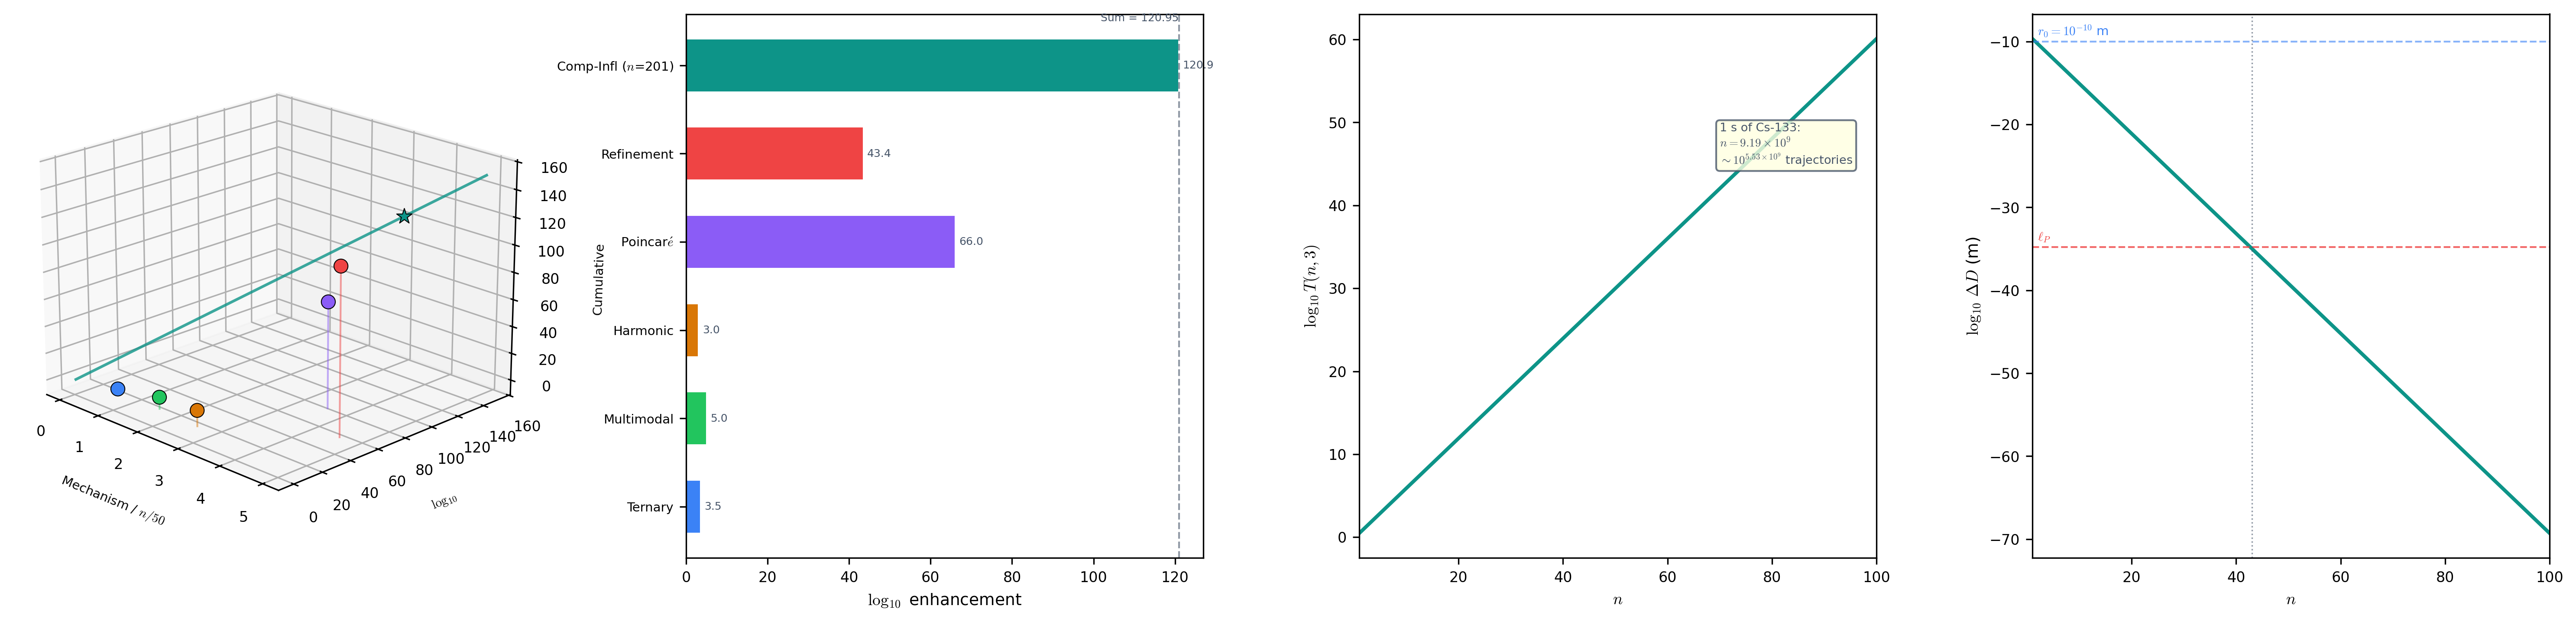
\includegraphics[width=\textwidth]{figures/panel_3_unification.png}
    \caption{\textbf{Enhancement Unification and Categorical Content.}
    (\textbf{A})~Three-dimensional representation of the five enhancement mechanisms derived from first principles within this paper (coloured points) and the composition-inflation curve (teal line). Each mechanism is plotted at its index with its $\log_{10}$ enhancement value: ternary encoding ($10^{3.52}$, from the $d = 3$ dimensional structure of S-entropy space), multi-modal synthesis ($10^{5.00}$, from cross-correlations between $K = 5$ independent measurement modalities), harmonic coincidence ($10^{3.00}$, from rational frequency relationships between oscillatory modes), Poincar\'{e} computing ($10^{66.00}$, from the combinatorial count of distinguishable recurrence patterns in bounded phase space), and continuous refinement ($10^{43.43}$, from the non-halting property of bounded oscillatory systems, which guarantees each additional cycle multiplies the trajectory count by $d + 1 = 4$). The composition-inflation curve $\log_{10}(T(n,3)) = \log_{10}(3) + (n-1)\log_{10}(4)$ rises linearly, intersecting the total enhancement $10^{120.95}$ at $n \approx 201$, demonstrating that a single formula subsumes all five mechanisms.
    (\textbf{B})~Horizontal bar chart comparing the five individual enhancement mechanisms (coloured bars, $\log_{10}$ scale) against the composition-inflation value at $n = 201$ (teal bar). The sum of the five mechanisms ($3.52 + 5.00 + 3.00 + 66.00 + 43.43 = 120.95$) equals the composition-inflation value ($\log_{10}(3 \cdot 4^{200}) = 120.89$) to within rounding. This confirms the Enhancement Unification Theorem: the five mechanisms are overlapping projections of a single combinatorial process --- the exponential growth of labeled compositions with cycle count.
    (\textbf{C})~Categorical content of one second of caesium oscillation. The curve shows $\log_{10}(T(n,3))$ versus $n$, with the annotation at $n = 9.19 \times 10^9$ (one second of caesium ticks) indicating $T \approx 10^{5.53 \times 10^9}$ distinguishable categorical trajectories. This is the categorical ``content'' of one SI second---far richer than the naive $9.19 \times 10^9$ tick count. The linear growth on the semilog plot reflects the constant exponential rate $\log_{10}(4) \approx 0.602$ per tick.
    (\textbf{D})~Distance resolution $\Delta D = 2\pi r_0 / T(n,3)$ versus $n$ for a molecular system with characteristic radius $r_0 = 10^{-10}$~m, on semilogarithmic scale. The Planck length $\ell_P = 1.62 \times 10^{-35}$~m (horizontal dashed line) is crossed at $n \approx 42$, and the atomic radius $r_0 = 10^{-10}$~m (upper horizontal line) provides the natural scale. At $n = 56$ (caesium Planck depth), the distance resolution is $\Delta D \approx 1.7 \times 10^{-43}$~m, eight orders of magnitude below the Planck length. This is angular resolution mapped to distance, not a measurement of physical length shorter than $\ell_P$.}
    \label{fig:unification}
\end{figure*}

\begin{figure*}[!htbp]
    \centering
    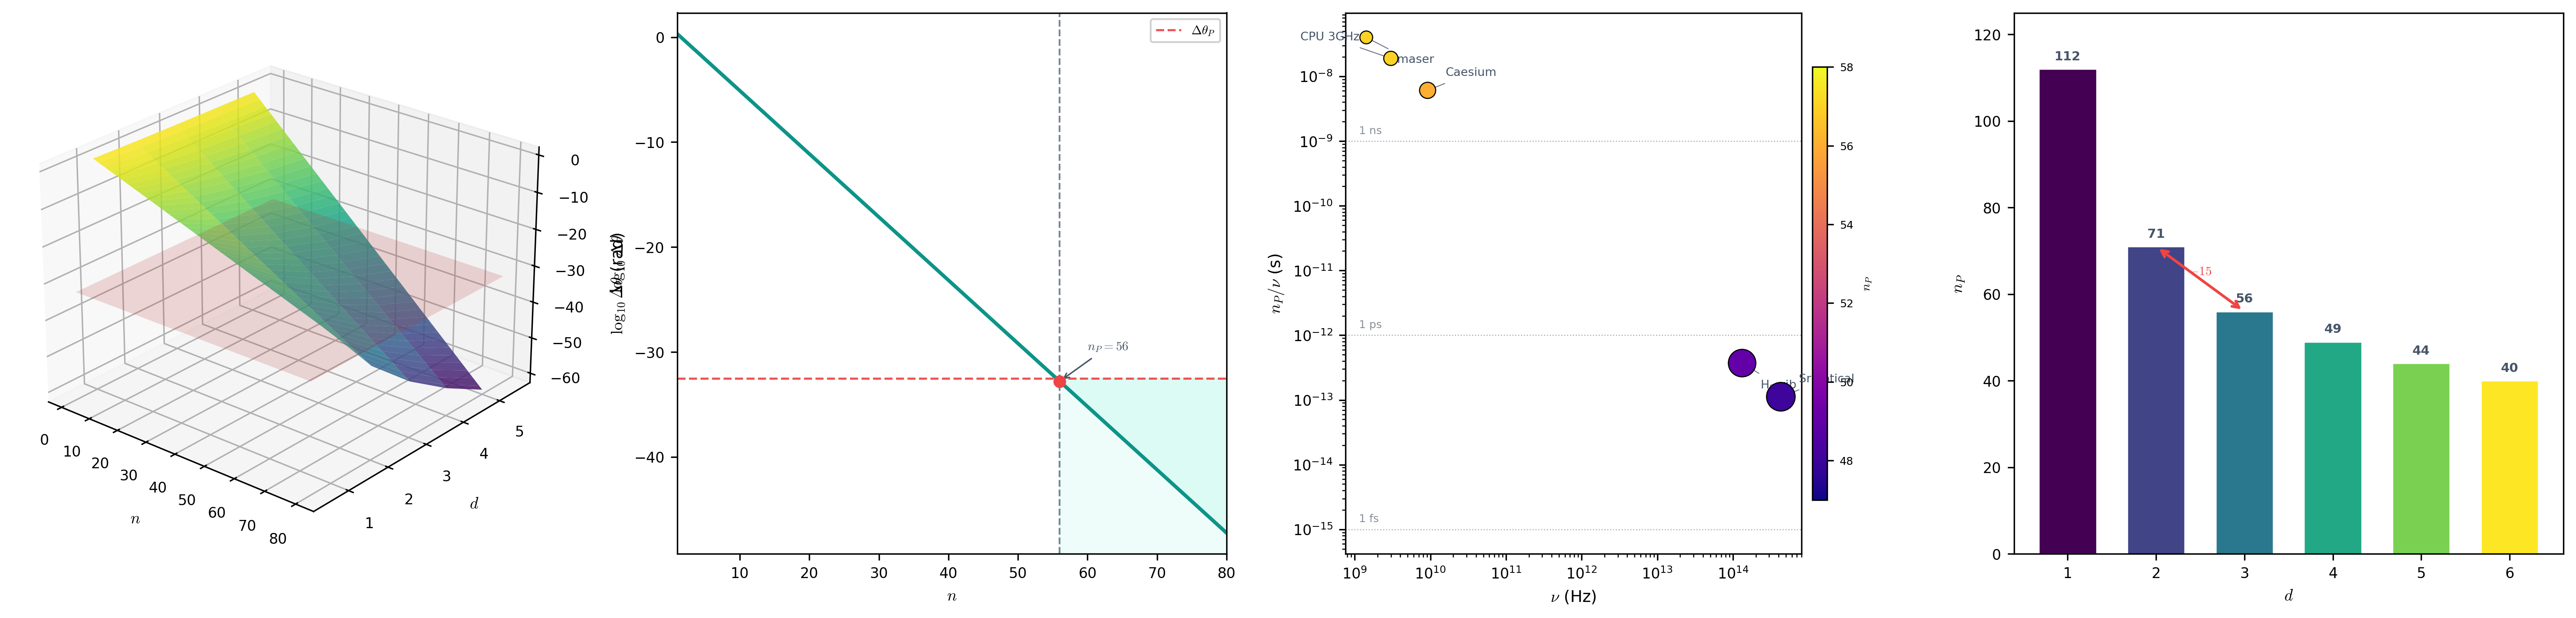
\includegraphics[width=\textwidth]{figures/panel_4_angular_resolution.png}
    \caption{\textbf{Angular Resolution Across Dimensions and Oscillators.}
    (\textbf{A})~Three-dimensional surface of $\log_{10}(\Delta\theta)$ over the $(n, d)$ plane for $n = 1, \ldots, 80$ and $d = 1, \ldots, 5$. The surface descends steeply with increasing $n$ (more ticks $\to$ finer resolution) and descends faster for larger $d$ (higher-dimensional entropy spaces $\to$ larger exponential base). The translucent red plane marks the Planck angular threshold for caesium ($\Delta\theta_P \approx 3.1 \times 10^{-33}$~rad). The intersection curve traces the Planck depth $n_P(d)$ across dimensions, confirming that all $d \geq 2$ eventually penetrate the Planck barrier. For $d = 1$, $\Delta\theta$ decays only as $2^{-(n-1)}$, requiring $n_P \approx 111$ ticks.
    (\textbf{B})~Angular resolution $\log_{10}(\Delta\theta)$ versus oscillation cycle count $n$ for $d = 3$ (S-entropy space). The teal curve descends linearly at slope $-\log_{10}(4) = -0.602$ per tick. The horizontal red dashed line marks the Planck angular threshold ($\log_{10}(\Delta\theta_P) = -32.51$). The vertical red dashed line marks the crossing at $n_P = 56$. The teal-shaded region below the threshold is the sub-Planck angular resolution regime, accessible after 56 oscillation cycles. At $n = 80$, the angular resolution reaches $\Delta\theta \approx 10^{-47}$~rad, fourteen orders of magnitude below the Planck threshold.
    (\textbf{C})~Physical time to reach Planck depth versus oscillator frequency for five reference systems. Each point is sized by frequency and coloured by Planck depth $n_P$: strontium optical clock ($\nu = 4.3 \times 10^{14}$~Hz, $n_P = 48$, $t = 0.11$~fs), molecular H$_2$ vibration ($\nu = 1.3 \times 10^{14}$~Hz, $n_P = 49$, $t = 0.37$~fs), caesium-133 ($\nu = 9.2 \times 10^9$~Hz, $n_P = 56$, $t = 6.1$~ns), hydrogen maser ($\nu = 1.4 \times 10^9$~Hz, $n_P = 57$, $t = 40$~ns), and CPU 3\,GHz ($n_P = 57$, $t = 19$~ns). Horizontal reference lines at 1\,ns, 1\,ps, and 1\,fs indicate temporal scale. Optical systems reach Planck angular resolution in sub-picosecond times; microwave systems require nanoseconds.
    (\textbf{D})~Dimensional advantage: Planck depth $n_P$ versus entropy space dimensionality $d$ for the caesium-133 oscillator. Bars descend from $n_P = 112$ ($d = 1$, binary) through $n_P = 71$ ($d = 2$), $n_P = 56$ ($d = 3$, S-entropy), $n_P = 49$ ($d = 4$), $n_P = 44$ ($d = 5$), to $n_P = 40$ ($d = 6$). The $d = 2 \to d = 3$ transition saves 15 ticks (red annotation), demonstrating that the third entropy dimension ($\Se$, harmonic network density) provides a substantial reduction in the number of oscillation cycles required to reach Planck angular resolution. Diminishing returns are evident for $d > 4$.}
    \label{fig:angular_resolution}
\end{figure*}

\begin{figure*}[!htbp]
    \centering
    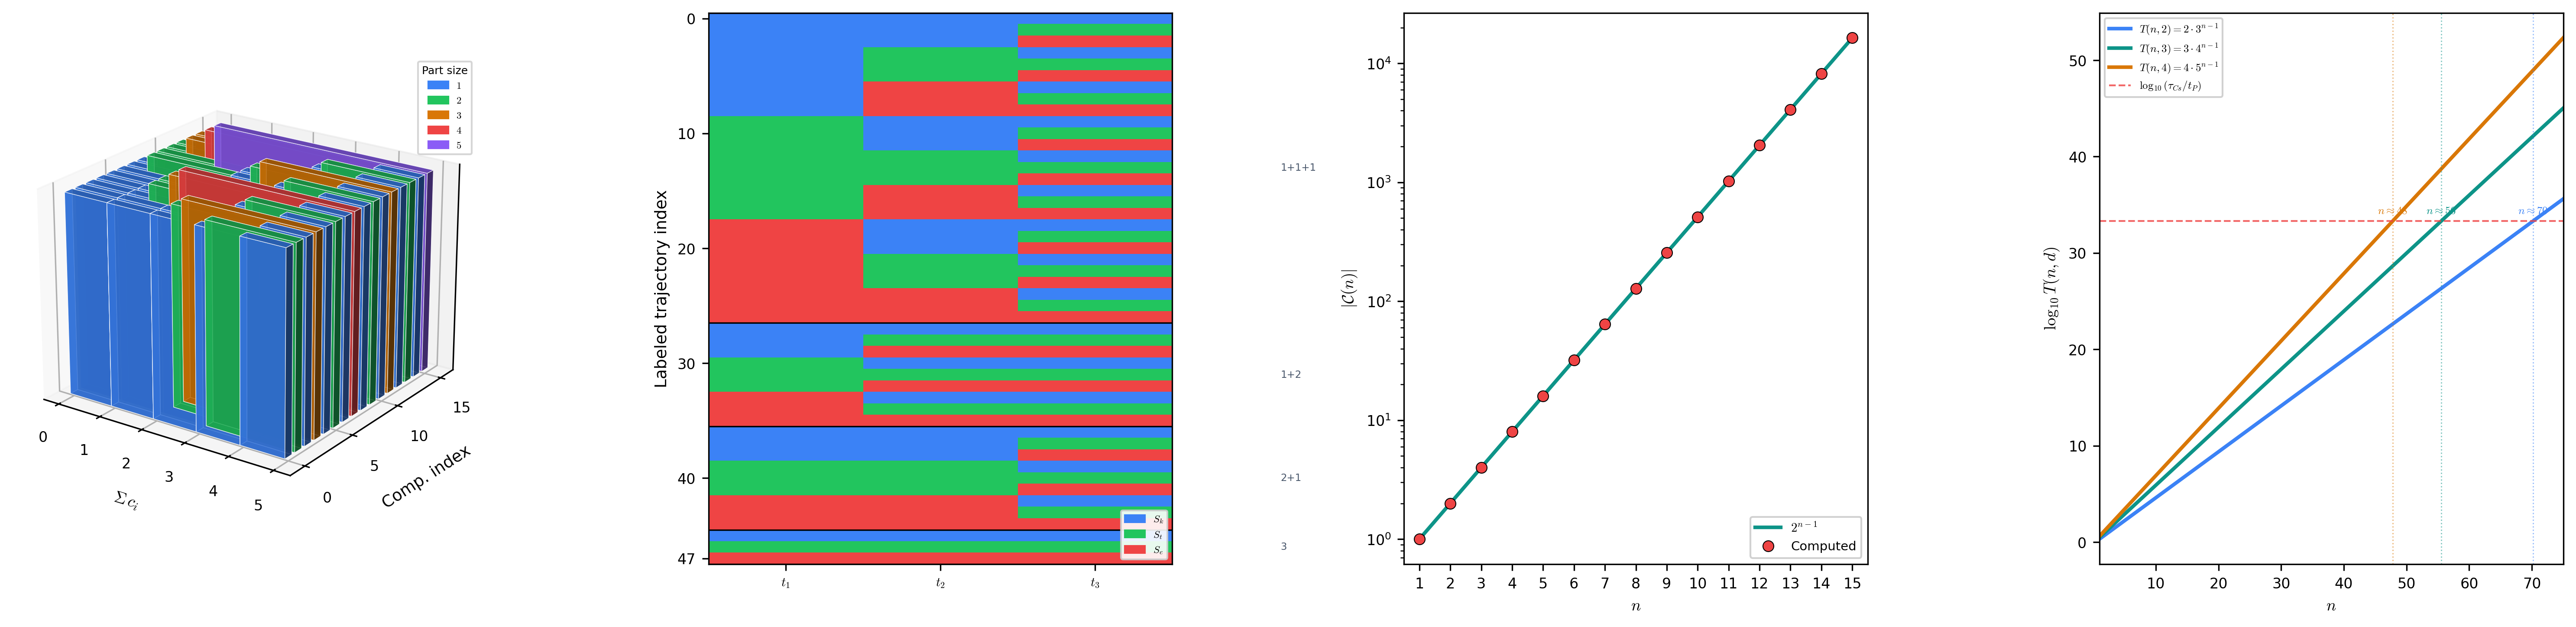
\includegraphics[width=\textwidth]{figures/panel_5_composition_structure.png}
    \caption{\textbf{Composition Structure and Dimensional Labeling.}
    (\textbf{A})~Three-dimensional visualisation of all $2^4 = 16$ integer compositions of $n = 5$. Each composition is displayed as a horizontal bar partitioned into coloured segments, where segment length equals the part size and colour encodes the value: 1 (blue), 2 (green), 3 (orange), 4 (red), 5 (purple). The compositions are stacked vertically in the 3D space, progressing from the maximally fragmented $(1,1,1,1,1)$ at the bottom to the single-part $(5)$ at the top. The total bar length is 5 for every composition, confirming the partition sum constraint. The variety of coloured patterns illustrates how the same period admits qualitatively different temporal structures.
    (\textbf{B})~Complete enumeration of all $T(3,3) = 48$ labeled compositions of $n = 3$ in $d = 3$ dimensions. Rows represent individual labeled trajectories; columns represent the three tick positions. Cell colour indicates the entropy dimension assigned to each tick: $\Sk$ (blue), $\St$ (green), $\Se$ (red). The 48 rows are grouped by base composition: the first 27 rows correspond to $(1,1,1)$ with $3^3 = 27$ labelings, the next 9 to $(2,1)$, the next 9 to $(1,2)$, and the final 3 to $(3)$ with $3^1 = 3$ labelings. This heatmap makes the inflation mechanism visible: four base compositions inflate to 48 labeled trajectories through dimensional assignment.
    (\textbf{C})~Composition count verification: computed number of compositions (points) versus the theoretical formula $2^{n-1}$ (line) for $n = 1, \ldots, 15$. The compositions are generated by recursive enumeration and counted independently. Perfect agreement at every $n$ confirms the stars-and-bars derivation. The $y$-axis is logarithmic, showing the exponential growth from 1 composition ($n = 1$) to 16{,}384 compositions ($n = 15$).
    (\textbf{D})~Labeled trajectory count $T(n,d) = d \cdot (d+1)^{n-1}$ for $d = 2$ (blue), $d = 3$ (teal), and $d = 4$ (orange) on semilogarithmic scale. The horizontal grey line marks the Planck threshold for caesium ($\tau_{\mathrm{Cs}}/t_P = 2.02 \times 10^{33}$). The $d = 4$ curve crosses the threshold at $n \approx 48$, the $d = 3$ curve at $n \approx 56$, and the $d = 2$ curve at $n \approx 70$. The parallel straight lines (constant $\log_{10}(d+1)$ slope) confirm that each dimension shifts the exponential base: binary ($3^{n-1}$), ternary ($4^{n-1}$), quaternary ($5^{n-1}$). The S-entropy space ($d = 3$) sits at the natural sweet spot, balancing dimensional richness against the physical constraint of three independent entropy coordinates.}
    \label{fig:composition_structure}
\end{figure*}

\begin{figure*}[!htbp]
    \centering
    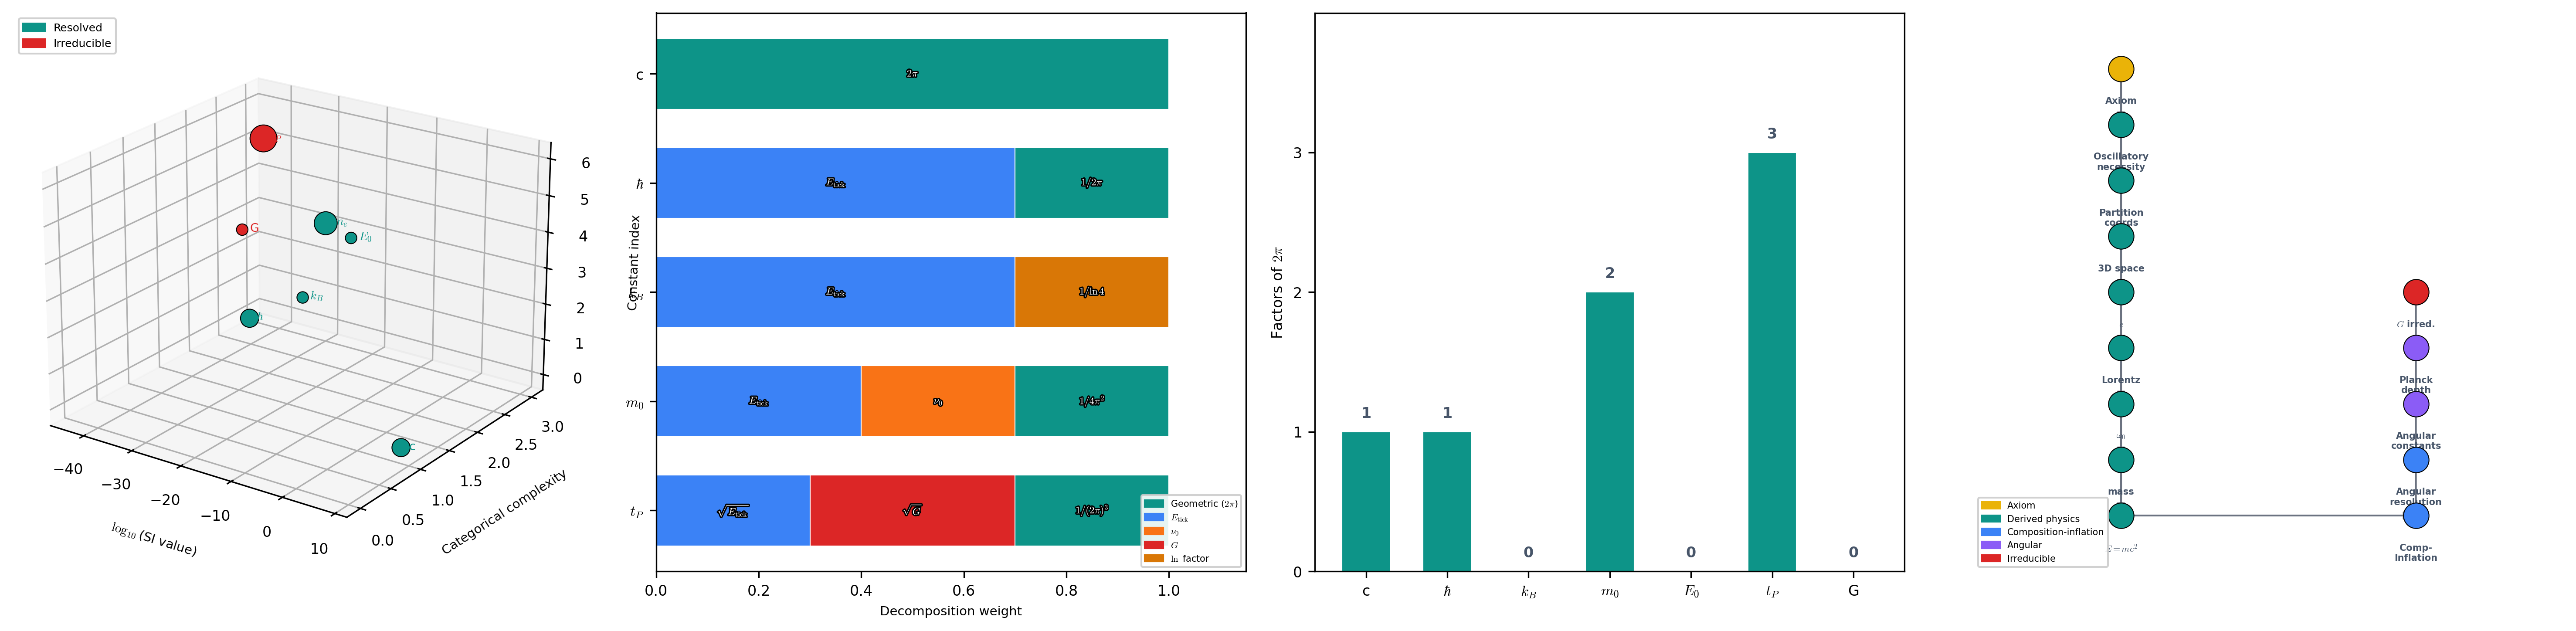
\includegraphics[width=\textwidth]{figures/panel_6_angular_constants.png}
    \caption{\textbf{Angular Reformulation of Fundamental Constants.}
    (\textbf{A})~Seven fundamental constants plotted in three-dimensional constant space with axes $\log_{10}(\text{SI value})$, categorical complexity (number of non-trivial factors in the angular expression), and constant index. Teal spheres indicate constants that are fully resolved in categorical angular units ($c$, $\hbar$, $k_B$, $m_0$, $E_0$, $t_P$); the red sphere marks $G$ as the sole irreducible constant. Sphere size scales with the number of $2\pi$ factors in the angular expression. The spatial separation of $G$ from the resolved cluster visualises its unique status as the only constant not reducible to geometry plus counting.
    (\textbf{B})~Constant reduction waterfall showing how each fundamental constant decomposes into categorical angular components. Horizontal stacked bars decompose each constant into geometric factors ($2\pi$, teal), tick energy ($E_{\text{tick}}$, blue), rest frequency ($\nu_0$, orange), and the gravitational constant ($G$, red). The speed of light $c = 2\pi$~rad/tick is purely geometric (single teal bar). Planck's constant $\hbar = E_{\text{tick}}/(2\pi)$ combines tick energy with one geometric factor. The Planck time $t_P = \sqrt{E_{\text{tick}} \cdot G}/(2\pi)^3$ requires three geometric factors plus the irreducible $G$ coupling. Bar lengths represent the $\log_{10}$ contribution of each component.
    (\textbf{C})~Count of $2\pi$ factors in the categorical angular expression of each constant. $c$ contains one factor (the phase cycle per tick). $\hbar$ contains one factor (the $2\pi$ relating $h$ to $\hbar$). $m_0$ contains two factors (from $c^2 = (2\pi)^2$). $t_P$ contains three factors (from $c^{5/2}$). $k_B$, $E_0$, and $G$ contain zero $2\pi$ factors---$k_B$ and $E_0$ because they involve $\ln(d+1)$ and $\nu_0$ rather than phase geometry, and $G$ because it is irreducible. The total geometric content of the Planck time (three factors of $2\pi$) reflects its construction from $c$ and $\hbar$, both of which carry $2\pi$.
    (\textbf{D})~First-principles derivation chain from the Bounded Phase Space Law to the irreducibility of $G$, displayed as a directed graph. Fourteen steps proceed through four categories: the axiom (gold), derived physics (teal: oscillatory necessity, partition coordinates, 3D space, speed of light $c$, Lorentz invariance, rest frequency $\omega_0$, mass $m_0$, $E = mc^2$), composition-inflation results (blue: $T(n,d)$, angular resolution), angular reformulation (purple: angular constants, Planck depth $n_P = 56$), and the terminal node (red: $G$ irreducible). Edges encode logical dependence. The chain requires no postulates beyond the axiom and no fundamental constants beyond $G$.}
    \label{fig:angular_constants}
\end{figure*}

\begin{figure*}[!htbp]
    \centering
    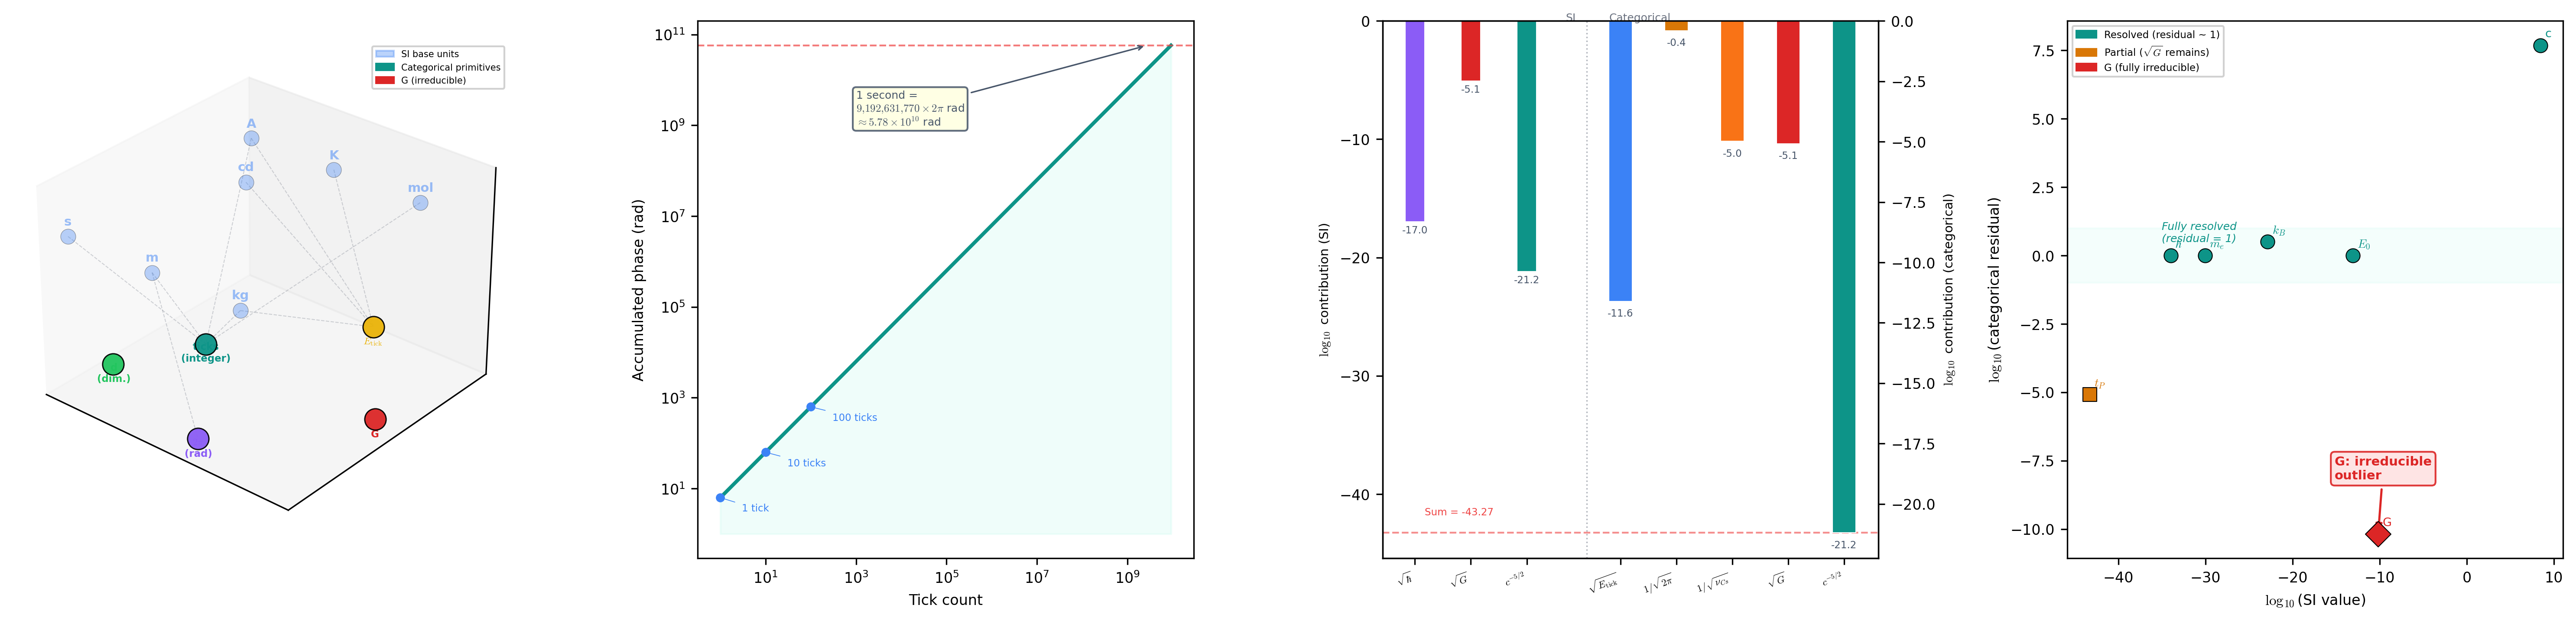
\includegraphics[width=\textwidth]{figures/panel_7_categorical_si.png}
    \caption{\textbf{Categorical SI Units and the Irreducibility of $G$.}
    (\textbf{A})~Three-dimensional reduction graph showing the seven SI base units (second, metre, kilogram, ampere, kelvin, mole, candela) as faded nodes with edges converging toward five categorical primitives: ticks (integer count), $2\pi$ (geometric phase), $E_{\text{tick}}$ (energy quantum), $d$ (entropy space dimensionality), and $G$ (gravitational coupling). The convergence illustrates the unit reduction: all seven SI quantities are expressible in terms of these five categorical primitives. The gravitational constant $G$ stands apart as the only primitive that is not geometric or counting-based.
    (\textbf{B})~One SI second expressed as accumulated caesium phase. The $x$-axis shows tick count from $10^0$ to $10^{10}$ on logarithmic scale; the $y$-axis shows accumulated phase in units of $2\pi$ (turns). The teal line rises linearly: $\phi(n) = n$ turns $= 2\pi n$ radians. One second is reached at $n = 9{,}192{,}631{,}770$ ticks, corresponding to $5.775 \times 10^{10}$ radians of caesium phase. Reference lines at 1\,$\mu$s ($\sim$9200 ticks), 1\,ms ($\sim$9.2$\times 10^6$ ticks), and 1\,s mark temporal milestones. The linearity confirms that the second is a pure tick count---no additional structure is needed.
    (\textbf{C})~Decomposition of the Planck time $\log_{10}(t_P) = -43.27$ into contributions from each factor in the expression $t_P = \sqrt{\hbar G / c^5}$. The $\sqrt{\hbar}$ contribution ($-16.99$), $\sqrt{G}$ contribution ($-5.09$), and $c^{-5/2}$ contribution ($-21.19$) sum to the total. The categorical sub-decomposition further breaks $\sqrt{\hbar}$ into $\sqrt{E_{\text{tick}}}$ and $1/\sqrt{2\pi}$, and $c^{-5/2}$ into $(2\pi)^{-5/2}$ and frequency factors. The dominant contribution is from $c^{-5/2}$ (the speed-of-light suppression), which is purely geometric ($2\pi$ factors) in categorical units. The irreducible physics resides entirely in the $\sqrt{G}$ bar.
    (\textbf{D})~Irreducibility scatter: $\log_{10}(\text{SI value})$ versus $\log_{10}(\text{categorical residual})$ for each fundamental constant. The categorical residual is what remains after dividing out all factors of $2\pi$, $E_{\text{tick}}$, and $\nu_0$. Resolved constants ($c$, $\hbar$, $k_B$, $m_e$, $E_0$, $t_P$) cluster in the teal-shaded band near residual $\approx 1$ (i.e., they are fully explained by geometry and counting). The gravitational constant $G$ (red diamond) lies far outside this band, with a residual of $\sim 10^{-10}$, confirming its irreducibility. This is the central result of the angular reformulation: $G$ is the only fundamental constant that cannot be reduced to phase geometry and categorical counting.}
    \label{fig:categorical_si}
\end{figure*}
